\chapter{O Estado da Arte: Observadores por Aprendizado Profundo, PCCT e Otimização Multiobjetivo}
\label{chap:estado_da_arte}

\section{Observadores Baseados em Aprendizado Profundo e Auto-Atenção}
\label{sec:dlmo}

Para superar a quebra de linearidade dos algoritmos DLR, a física médica desenvolveu os Observadores de Modelo Baseados em Aprendizado Profundo (\emph{Deep Learning Model Observers} --- DLMO) \cite{zhou2021, schilder2026}.

Em vez de assumir templates lineares fixos, o DLMO emprega redes neurais profundas com arquitetura \emph{Vision Transformer} (ViT) dotadas de mecanismos de Auto-Atenção Multi-Cabeça (MHSA), conforme esquematizado no \cref{fig:dlmo_arch}.

\begin{figure}[htbp]
  \centering
  
\includegraphics[width=0.95\textwidth]{figuras/flow5_dlmo_architecture.png}
  \caption{Arquitetura Neural do Observador por Aprendizado Profundo (DLMO) com Auto-Atenção Multi-Cabeça (Vision Transformer) e Calibração Perceptual.}
  \label{fig:dlmo_arch}
\end{figure}

\subsection{Arquitetura Vision Transformer: Projeção Linear e Patch Embeddings}
A imagem tomográfica $\mathbf{x} \in \mathbb{R}^{H \times W \times C}$ é dividida em uma sequência de $N_p = \frac{HW}{P^2}$ blocos bidimensionais não-sobrepostos (\emph{patches}) $\mathbf{x}_p \in \mathbb{R}^{N_p \times (P^2 C)}$, onde $P \times P$ é a dimensão espacial de cada bloco \cite{dosovitskiy2021}. Cada bloco é projetado linearmente para um espaço latente de dimensão $D_{\text{model}}$ através de uma matriz treinável $\mathbf{E}$:
\begin{equation}
  \mathbf{z}_0 = \left[ \mathbf{x}_{\text{class}}; \, \mathbf{x}_p^1 \mathbf{E}; \, \mathbf{x}_p^2 \mathbf{E}; \, \dots; \, \mathbf{x}_p^{N_p} \mathbf{E} \right] + \mathbf{E}_{\text{pos}}
  \label{eq:vit_embedding}
\end{equation}
onde $\mathbf{x}_{\text{class}}$ é o token especial de decisão e $\mathbf{E}_{\text{pos}} \in \mathbb{R}^{(N_p + 1) \times D_{\text{model}}}$ codifica as coordenadas espaciais 2D absolutas.

\subsection{Mecanismo de Auto-Atenção Multi-Cabeça e Conexão Neurofisiológica}
A auto-atenção permite à rede computacional aprender correlações espaciais globais e locais simultaneamente. Para cada bloco, calculam-se as projeções de Consulta ($Q$), Chave ($K$) e Valor ($V$):
\begin{equation}
  Q = \mathbf{z} \mathbf{W}_Q, \qquad K = \mathbf{z} \mathbf{W}_K, \qquad V = \mathbf{z} \mathbf{W}_V
  \label{eq:qkv}
\end{equation}

A equação de auto-atenção escalonada por produto escalar é expressa por:
\begin{equation}
  \text{Attention}(Q, K, V) = \text{softmax}\left( \frac{Q K^T}{\sqrt{d_k}} \right) V
  \label{eq:attention_formula}
\end{equation}
onde o fator $\sqrt{d_k}$ evita a saturação dos gradientes na função softmax.

Do ponto de vista neurofisiológico, essa formulação matemática mimetiza a interação foveal-periférica dos radiologistas: a matriz de atenção pondera áreas anatômicas distantes para inferir o contexto anatômico de fundo enquanto focaliza recursos computacionais na detecção foveal da lesão central.

A estatística de teste não linear $t_{\text{DL}}(\mathbf{g}) = f_{\boldsymbol{\theta}}(\mathbf{g})$ permite calcular o índice de detectabilidade não linear:
\begin{equation}
  d'_{\text{DL}} = \frac{\langle f_{\boldsymbol{\theta}}(\mathbf{g}) | H_1 \rangle - \langle f_{\boldsymbol{\theta}}(\mathbf{g}) | H_0 \rangle}{\sqrt{\frac{1}{2}\sigma^2(f_{\boldsymbol{\theta}}(\mathbf{g})|H_1) + \frac{1}{2}\sigma^2(f_{\boldsymbol{\theta}}(\mathbf{g})|H_0)}}
  \label{eq:dprime_dl}
\end{equation}

\section{Calibração Perceptual com Radiologistas e Transferibilidade Leave-One-Scanner-Out}
\label{sec:loso}

Para que o modelo DLMO funcione como um instrumento metrológico clinicamente representativo, ele não deve ser treinado apenas como um classificador matemático puro, mas sim calibrado através de uma função de perda perceptual multitarefa ancorada em leituras humanas:
\begin{equation}
  \mathcal{L}_{\text{total}}(\boldsymbol{\theta}) = \mathcal{L}_{\text{classificação}}(y, \hat{y}) + \lambda \, \left( d'_{\text{DL}}(\boldsymbol{\theta}) - d'_{\text{humano}} \right)^2
  \label{eq:perceptual_loss}
\end{equation}
onde $\mathcal{L}_{\text{classificação}}$ garante a acurácia na separação de classes e o segundo termo penaliza desvios em relação à detectabilidade medida no painel de radiologistas em testes 2AFC.

A capacidade de generalização do modelo é testada pelo método \emph{Leave-One-Scanner-Out} (LOSO), onde a rede é treinada com dados de $K - 1$ tomógrafos e testada cegamente no tomógrafo restante, garantindo robustez inter-institucional.

\section{Física da Tomografia Computadorizada por Contagem de Fótons}
\label{sec:pcct_fisica}

A Tomografia Computadorizada por Contagem de Fótons (\emph{Photon-Counting CT} --- PCCT) representa o salto tecnológico mais expressivo da tomografia na última década \cite{flohr2020, mccollough2026, pimenta2025, pimenta2026}.

A \cref{tab:eict_vs_pcct} sintetiza as diferenças fundamentais entre a tecnologia clássica (EICT) e os detectores de contagem de fótons (PCCT).

\begin{table}[htbp]
  \centering
  \small
  \caption{Comparativo físico entre as tecnologias de detecção tomográfica EICT e PCCT.}
  \label{tab:eict_vs_pcct}
  \begin{tabularx}{\textwidth}{lXX}
    \toprule
    \textbf{Característica Física} & \textbf{TC por Integração de Energia (EICT)} & \textbf{TC por Contagem de Fótons (PCCT)} \\
    \midrule
    \textbf{Material Detector} & Cintilador cerâmico ($\text{Gd}_2\text{O}_2\text{S}$) + Fotodiodo & Semicondutor de conversão direta (CdTe / CZT / Silício) \\
    \textbf{Mecanismo de Conversão} & Indireta: Raios X $\to$ Luz visível $\to$ Carga elétrica & Direta: Raios X $\to$ Pares elétron-lacuna instantâneos \\
    \textbf{Ruído Eletrônico} & Integrado cumulativamente ao sinal de raios X & Rejeitado por limiar inferior de energia ($E_{\text{threshold}} > E_{\text{ruído}}$) \\
    \textbf{Resolução Espacial} & Limitada por septos ópticos refletivos ($0{,}5 \text{ a } 0{,}6 \text{ mm}$) & Submilimétrica ultra-alta ($0{,}1 \text{ a } 0{,}2 \text{ mm}$, sem septos físicos) \\
    \textbf{Ponderação Espectral} & Proporcional à energia do fóton ($S \propto E$, subpondera baixa energia) & Contagem individual com peso unitário ou peso ideal ótimo \\
    \textbf{Capacidade Espectral} & Requer duas fontes/camadas de detectores & Intrínseca: Múltiplos canais de energia (\emph{energy bins}) em único disparo \\
    \bottomrule
  \end{tabularx}
\end{table}

\subsection{Detectores Semicondutores de Conversão Direta: CdTe versus Silício}
Enquanto os detectores tradicionais EICT dependem da conversão de raios X em luz visível dentro de cristais cintiladores cerâmicos (processo que induz espalhamento óptico e exige septos refletores entre pixels), os detectores PCCT utilizam cristais semicondutores espessos (de 1,5 a 3,0 mm de Telureto de Cádmio --- CdTe, CZT ou Silício polarizados sob alta tensão de -800 V a -1000 V). A absorção fotoelétrica de cada fóton incidente gera imediatamente uma nuvem de pares elétron-lacuna que migra em nanossegundos em direção aos ânodos pixelados, produzindo um pulso elétrico cuja amplitude de corrente é estritamente proporcional à energia do fóton:
\begin{equation}
  V_{\text{pulso}} \propto Q = \frac{E_{\text{fóton}}}{W_{\text{ionização}}}
  \label{eq:vpulso}
\end{equation}
onde $W_{\text{ionização}} \approx 4{,}43 \text{ eV}$ para o CdTe (comparado aos $30 \text{ eV}$ necessários para gerar um elétron em cintiladores convencionais).

\subsection{Fenômenos Estocásticos: Charge Sharing e Pulse Pile-Up}
Apesar de sua eficiência, dois fenômenos estocásticos complexos desafiam a modelagem metrológica em PCCT:
\begin{enumerate}
  \item \textbf{Compartilhamento de Carga (\emph{Charge Sharing}):} Quando um fóton de raios X interage próximo à borda entre dois micropixels, a nuvem de elétrons em expansão divide-se entre ânodos adjacentes, gerando múltiplos pulsos de menor amplitude (\emph{charge splitting}). Sistemas avançados compensam esse efeito através de circuitos de adição de carga em tempo real (\emph{Charge-Sharing Correction});
  \item \textbf{Empilhamento de Pulsos (\emph{Pulse Pile-Up}):} Em altas taxas de exposição tomográfica ($> 10^7 \text{ fótons}/(\text{mm}^2\cdot\text{s})$), múltiplos fótons atingem o mesmo pixel antes que o circuito integrador retorne à linha de base, causando contagens subestimadas e distorções espectrais na altura do pulso.
\end{enumerate}

\subsection{Compartimentalização de Energia e Imagens Monoenergéticas Virtuais}
A discriminação eletrônica dos pulsos em múltiplos comparadores com limiares de energia programáveis ($E_1, E_2, E_3, E_4$) permite a decomposição das projeções tomográficas na base de materiais fundamentais (efeito fotoelétrico e espalhamento Compton), viabilizando a síntese de Imagens Monoenergéticas Virtuais ($VMI$) em qualquer energia nominal desejada (de 40 a 140 keV):
\begin{equation}
  I_{\text{VMI}}(x, y; E_0) = a_1(x, y) \cdot f_{\text{foto}}(E_0) + a_2(x, y) \cdot f_{\text{Compton}}(E_0)
  \label{eq:vmi_formula}
\end{equation}

Em baixas energias nominais ($40 \text{ a } 50 \text{ keV}$), maximiza-se a absorção fotoelétrica do iodo ($K\text{-edge} = 33{,}2 \text{ keV}$), elevando substancialmente a $TTF$ de pequenas lesões vasculares e neoplásicas. Como a PCCT rejeita totalmente o ruído eletrônico, é possível sintetizar imagens de 40 keV sem a explosão de ruído estocástico que inviabilizava essa técnica nos tomógrafos EICT convencionais.

\section{Otimização Multiobjetivo em TC: A Fronteira de Pareto Tridimensional}
\label{sec:pareto_otimizacao}

A otimização tradicional de protocolos limitava-se a buscar o equilíbrio entre dose e qualidade de imagem. Contudo, em ambientes hospitalares de alta rotatividade (prontos-socorros e centros de trauma), o tempo operacional total ($T = T_{\text{aq}} + T_{\text{rec}}$) é uma variável determinante \cite{oostveen2021}.

A física médica moderna modela esse cenário como um problema de Otimização Multiobjetivo Não Linear:
\begin{equation}
  \min_{\mathbf{p} \in \Omega} \mathbf{F}(\mathbf{p}) = \begin{pmatrix} D(\mathbf{p}) \\ T(\mathbf{p}) \\ -W(\mathbf{p}) \end{pmatrix}
  \label{eq:multiobjetivo_pareto}
\end{equation}
sujeito às restrições clínicas formais:
\begin{itemize}
  \item $D(\mathbf{p}) \le \text{DRL}$ (restrição de dose de radioproteção);
  \item $T(\mathbf{p}) \le T_{\text{máx}}$ (restrição operacional de tempo em emergência);
  \item $W(\mathbf{p}) = d'(\mathbf{p}) \ge d'_{\text{mín}}$ (restrição diagnóstica de detectabilidade).
\end{itemize}

A \cref{fig:pareto_3d} apresenta o mapeamento da Fronteira de Pareto nos domínios bidimensional e tridimensional.

\begin{figure}[htbp]
  \centering
  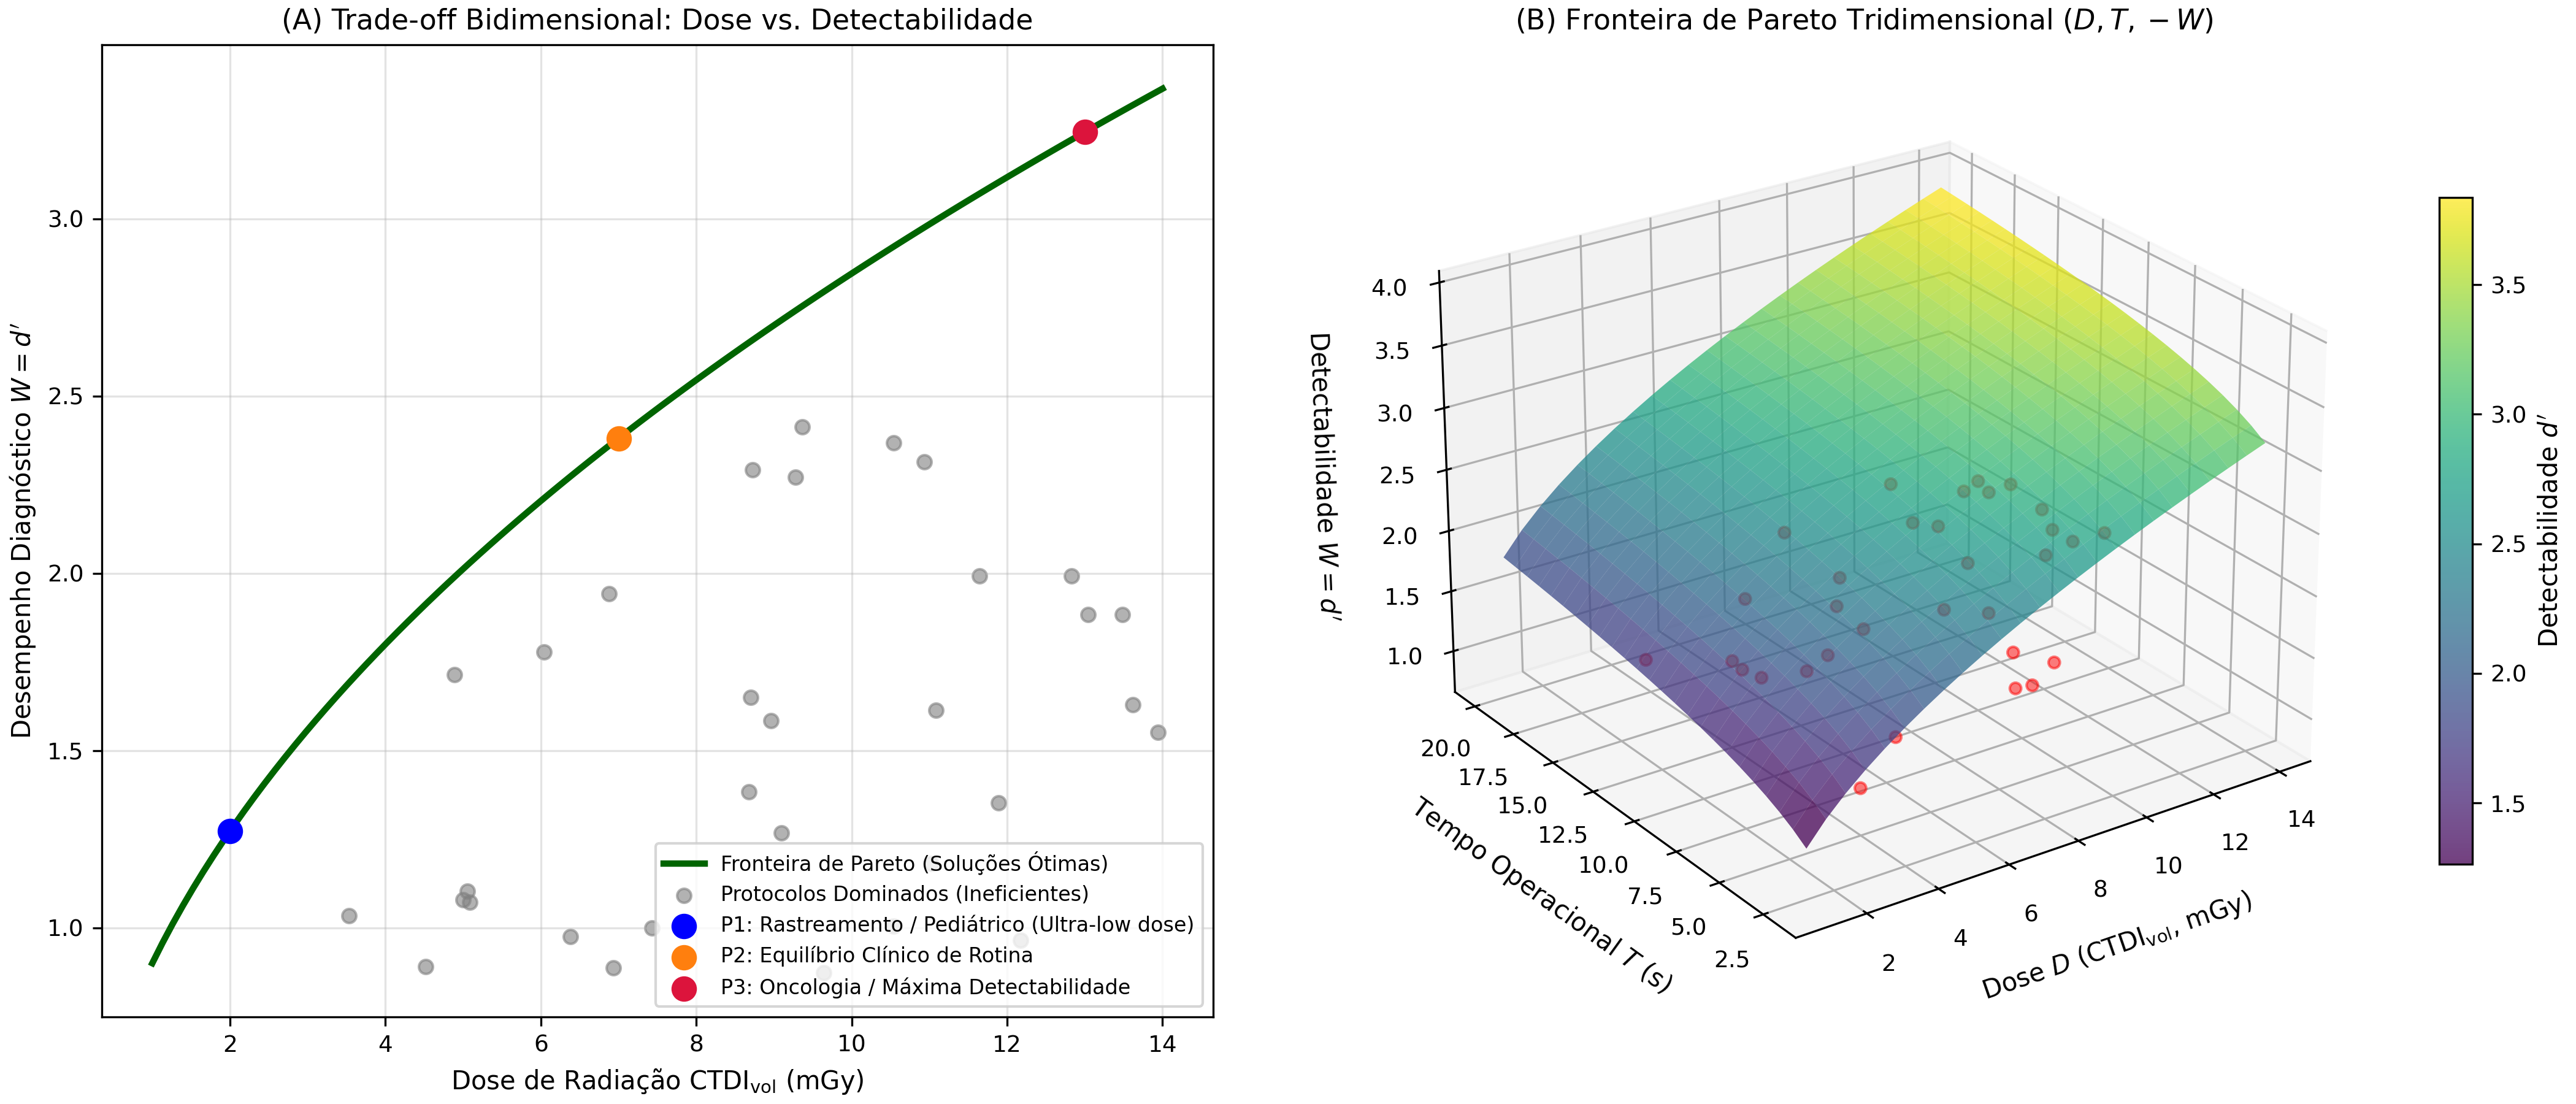
\includegraphics[width=0.98\textwidth]{figuras/fig5_dlmo_pareto_3d.png}
  \caption{Otimização Multiobjetivo em Tomografia Computadorizada e Fronteira de Pareto. (A) Trade-off bidimensional entre Dose e Detectabilidade, ilustrando soluções ótimas na fronteira e protocolos dominados ineficientes. (B) Fronteira de Pareto Tridimensional $(D, T, -W)$, integrando Dose de Radiação ($D$), Tempo Operacional total ($T$) e Detectabilidade Diagnóstica ($W = d'$).}
  \label{fig:pareto_3d}
\end{figure}

O mapeamento dessa superfície de soluções não-dominadas é realizado através do Algoritmo Genético NSGA-II acoplado ao método de tomada de decisão multicritério TOPSIS, permitindo escolher o protocolo ótimo para cada perfil institucional (pediátrico de ultrabaixa dose, emergência ultrarrápida ou oncologia de alta resolução).
